\documentclass{rapportFSR}
\usepackage[utf8]{inputenc}
\usepackage{lipsum}
\usepackage{minted}
\usepackage{mdframed}
\usepackage{tcolorbox}
\usepackage{pifont}
\usepackage{fontawesome5}
\usepackage{listings}
\usepackage{xcolor}

\usepackage{colortbl}

\lstdefinestyle{console}{
    backgroundcolor=\color{black!5},
    basicstyle=\ttfamily\small,
    frame=single,
    columns=fullflexible
}

\definecolor{bg}{rgb}{0.95,0.95,0.95} 

\title{Rapport FSR - Template}

\begin{document}

%------------------ Informations du TP (à remplir) ------------------
\titre{Compte Rendu de TP 1} 
\sujet{Nom du module} 
\enseignant{Pr. Prénom \textsc{NOM}} 
\eleves{Prénom \textsc{NOM}} 

\fairemarges
\fairepagedegarde
\tabledematieres
\newpage
\listoffigures
\newpage

%------------------ Section 1 ------------------
\section{Exercice 1 – Titre de l’exercice}

Présentez en quelques lignes l’objectif de l’exercice et l’environnement utilisé.

\subsection{Première manipulation}

Décrivez ce que vous faites et pourquoi.

\begin{lstlisting}[style=console]
$ commande --option argument
\end{lstlisting}

\begin{figure}[H]
    \centering
    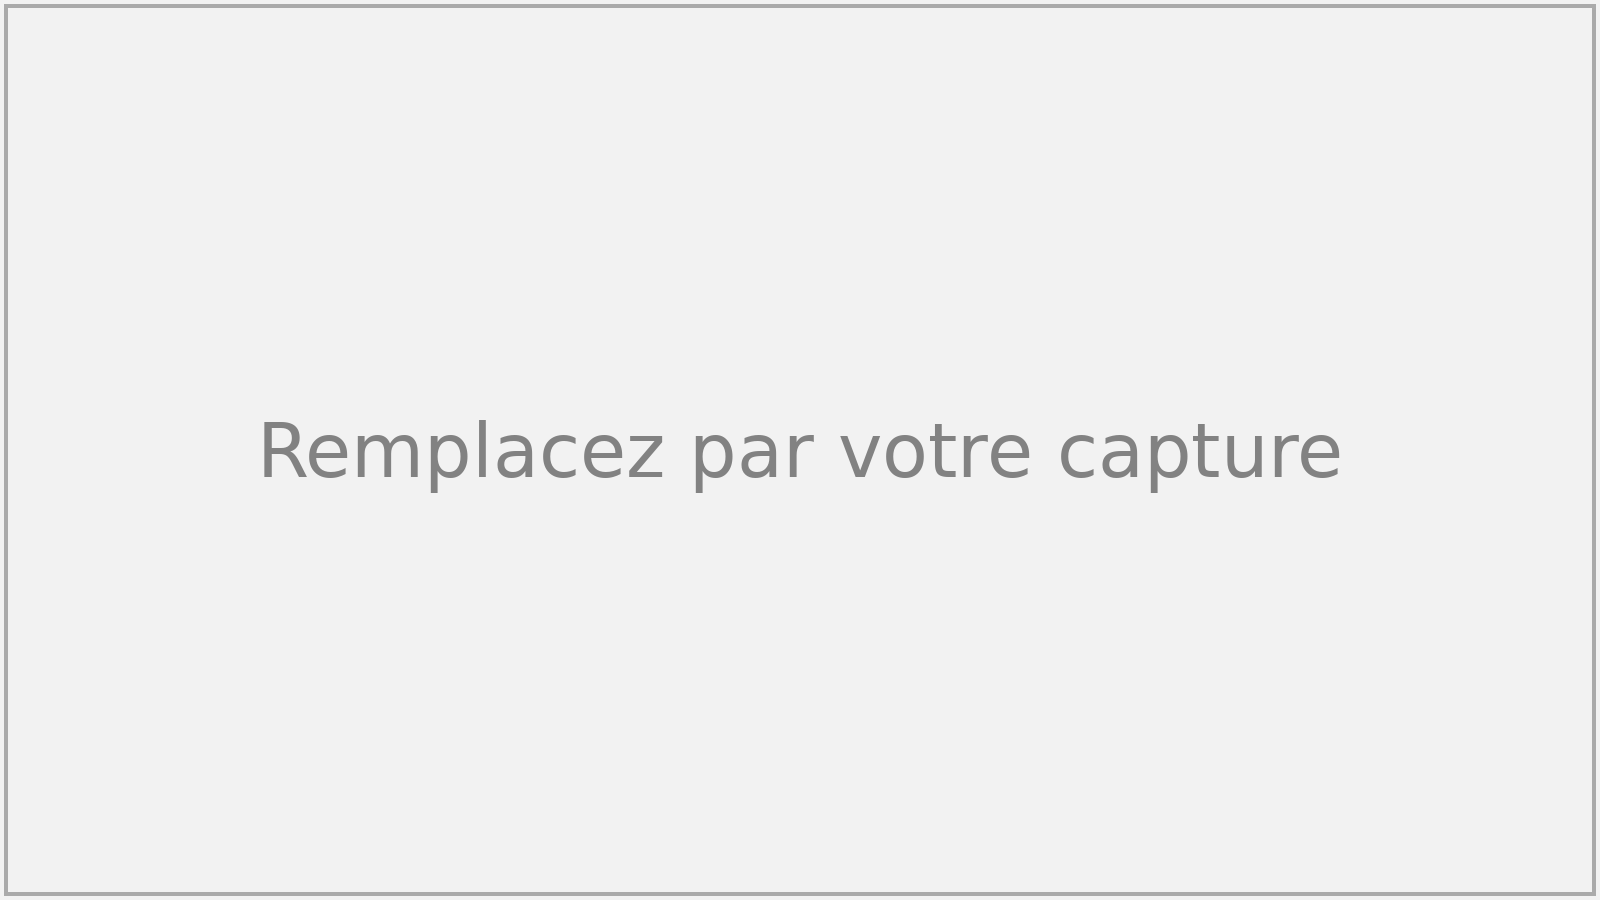
\includegraphics[width=0.75\linewidth]{capture.png}
    \caption{Titre de la capture}
    \label{fig:ex1-manip1}
\end{figure}

\subsection{Deuxième manipulation}

\begin{figure}[H]
    \centering
    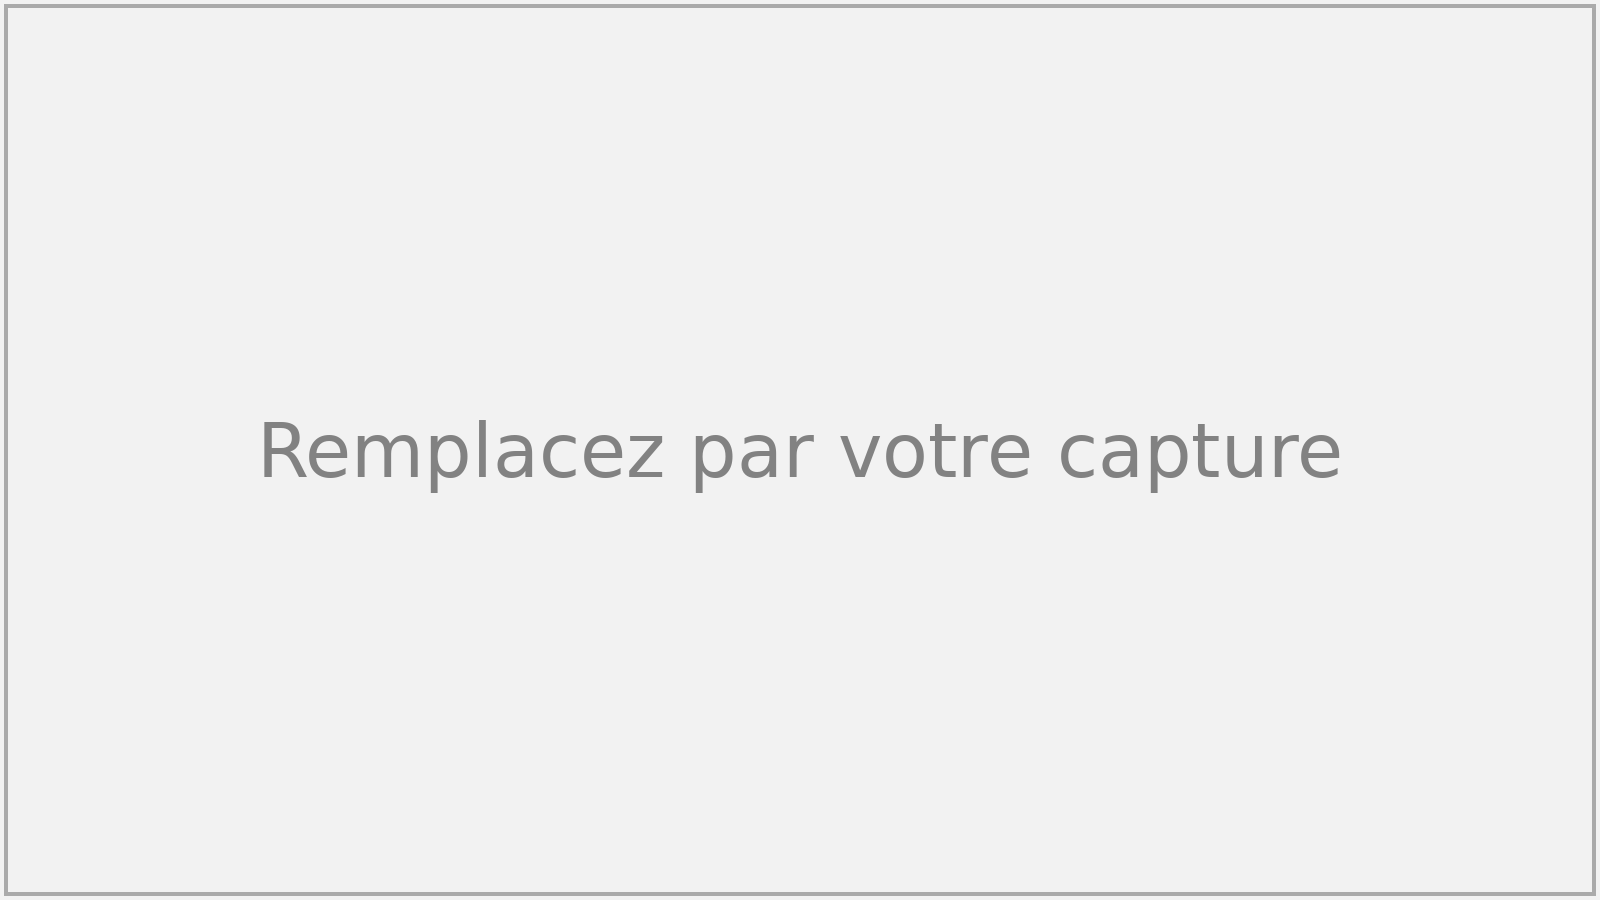
\includegraphics[width=0.75\linewidth]{capture.png}
    \caption{Titre de la capture}
    \label{fig:ex1-manip2}
\end{figure}

\subsection{Questions}

\textbf{1. Recopiez ici la question de l’énoncé ?} \\
Votre réponse.

\textbf{2. Recopiez ici la question de l’énoncé ?} \\
Votre réponse.

%------------------ Section 2 ------------------
\section{Exercice 2 – Titre de l’exercice}

\subsection*{Exemples de commandes utilisées}

Les commandes suivantes font partie des opérations abordées dans cet exercice.

\definecolor{header}{RGB}{40,60,120}
\definecolor{rowgray}{RGB}{245,245,245}
\definecolor{lightblue}{RGB}{225,235,255}

\begin{table}[H]
\centering
\rowcolors{2}{rowgray}{white}
\begin{tabular}{|p{4cm}|p{10cm}|}
\hline
\rowcolor{header}
\textcolor{white}{Commande} &
\textcolor{white}{Description} \\
\hline

\rowcolor{lightblue}
\multicolumn{2}{|l|}{\textbf{Catégorie 1}} \\
\hline
commande 1 & Description de la commande. \\
commande 2 & Description de la commande. \\
\hline

\rowcolor{lightblue}
\multicolumn{2}{|l|}{\textbf{Catégorie 2}} \\
\hline
commande 3 & Description de la commande. \\
commande 4 & Description de la commande. \\
\hline

\end{tabular}
\caption{Commandes utilisées}
\end{table}

\subsection{Manipulation}

\begin{lstlisting}[style=console]
$ commande --option argument
\end{lstlisting}

\begin{figure}[H]
    \centering
    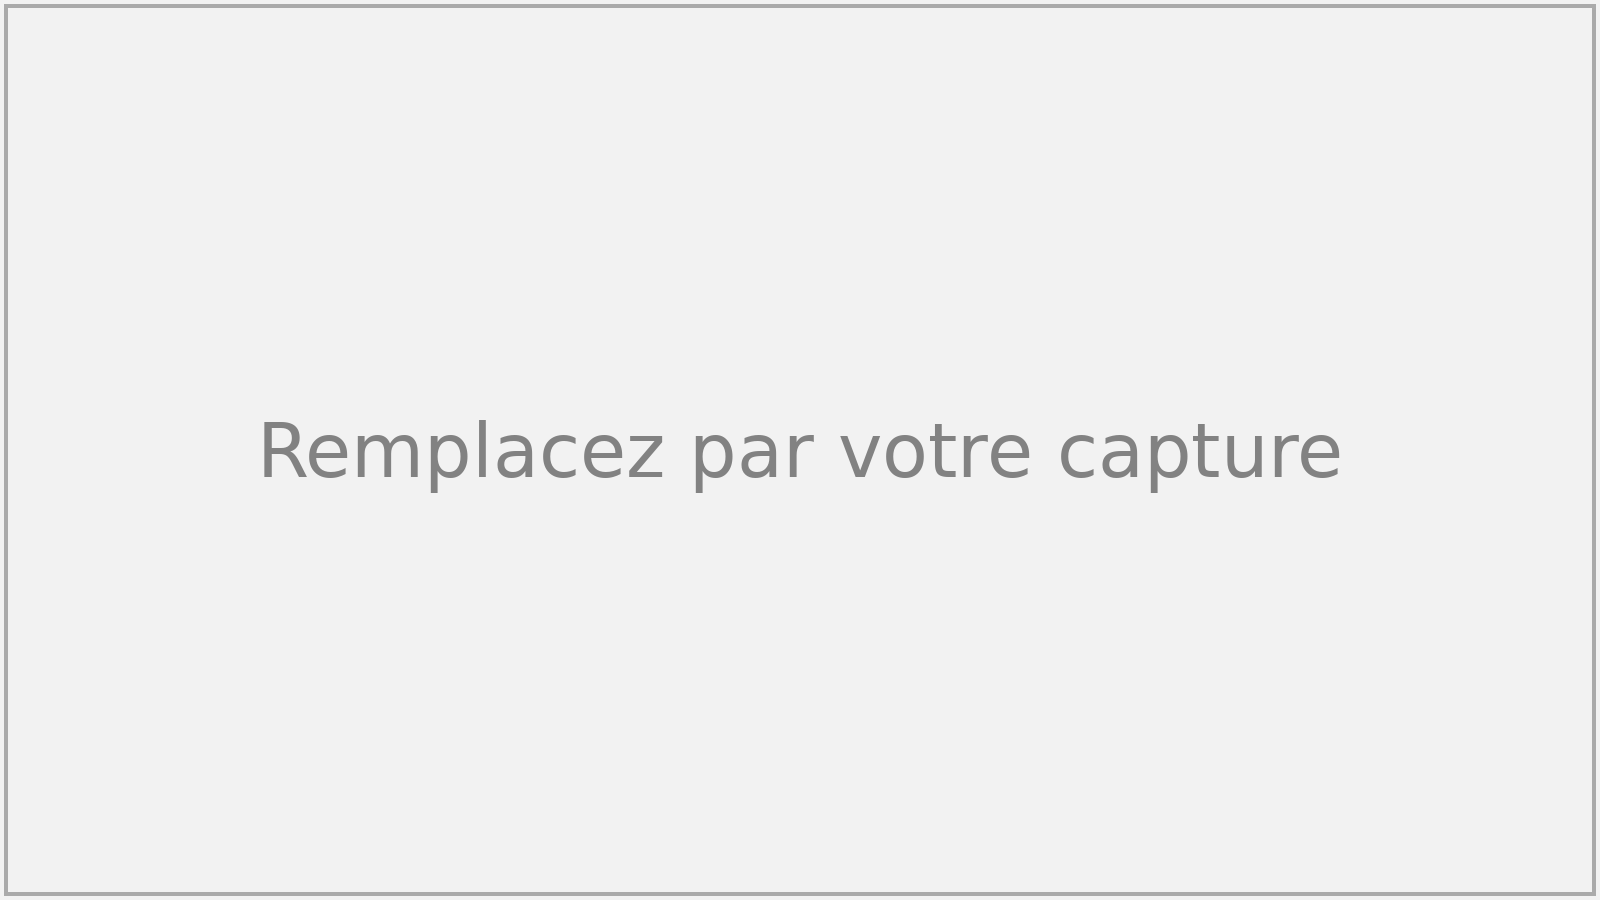
\includegraphics[width=0.75\linewidth]{capture.png}
    \caption{Titre de la capture}
    \label{fig:ex2-manip1}
\end{figure}

\subsection{Questions}

\textbf{3. Recopiez ici la question de l’énoncé ?} \\
Votre réponse.

%------------------ Section 3 ------------------
\section{Bonus (optionnel) : Titre}

\begin{figure}[H]
    \centering
    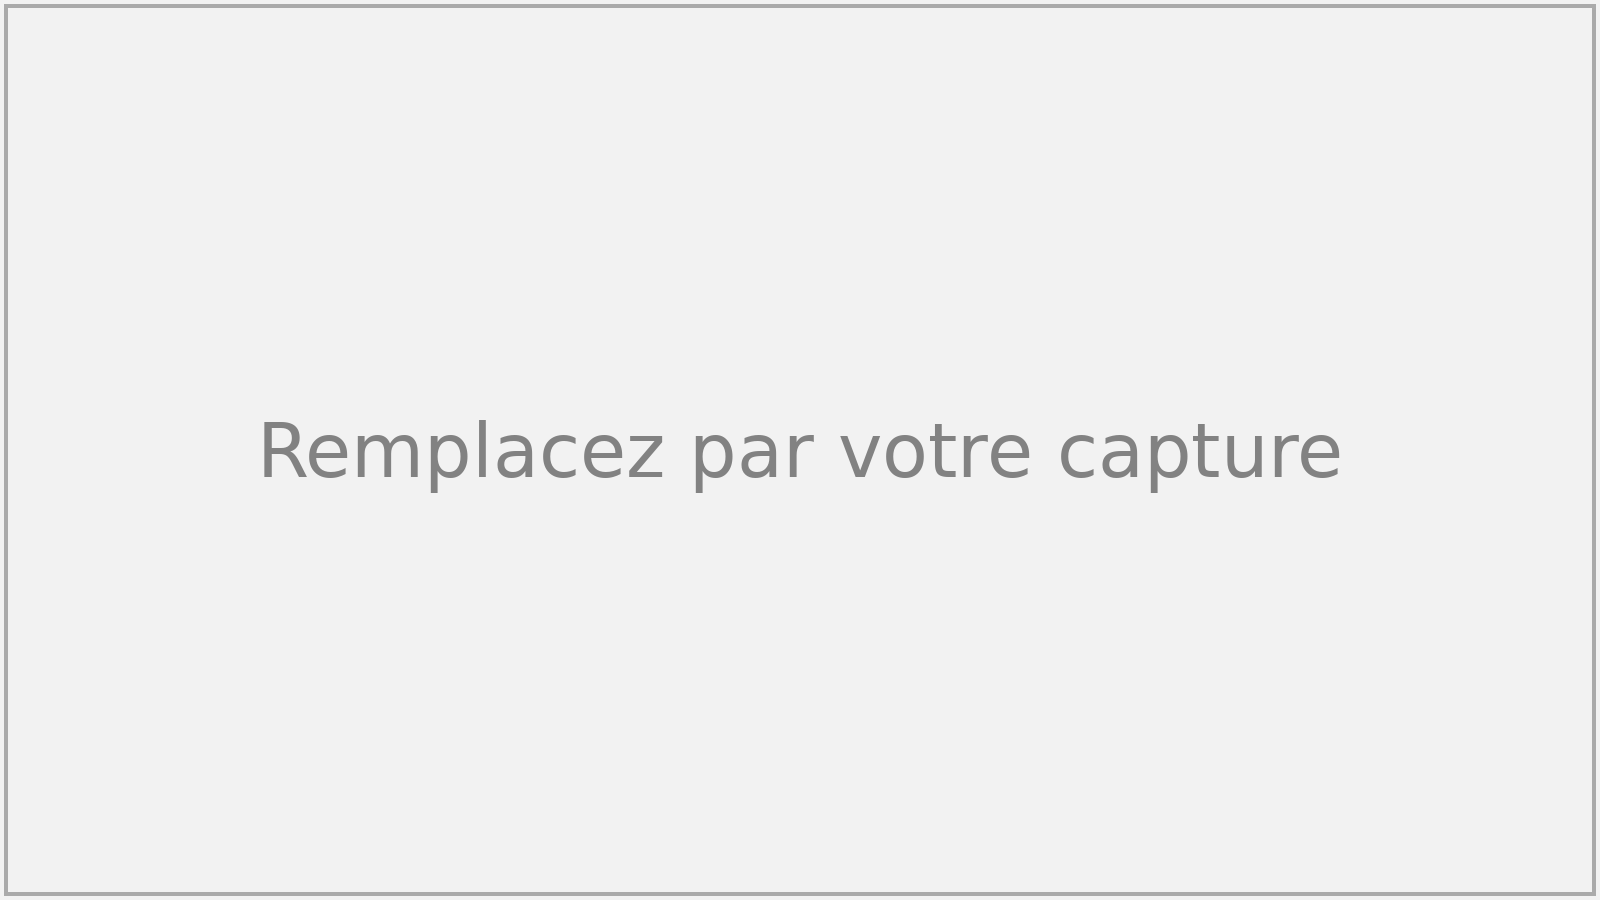
\includegraphics[width=0.75\linewidth]{capture.png}
    \caption{Titre de la capture}
    \label{fig:bonus}
\end{figure}

\subsection{Questions}

\textbf{4. Recopiez ici la question de l’énoncé ?} \\
Votre réponse.

\end{document}
